\chapter{Metamodelling}
\label{metamodellingChapter}

\section{Introduction}

The previous chapter described the benefits of using semantically
rich languages to precisely capture, relate and manipulate
different aspects of a problem domain. These languages may be
general purpose languages, domain specific languages, modelling
languages or programming languages. In order to realise these
benefits, a way must be found of defining languages in a unified
and semantically rich way. In this chapter we begin exploring a
means of achieving this using {\em metamodels}.

This chapter sets out to explain a number of key aspects of
metamodelling that lay the foundation for the rest of this book.
An important starting point is to understand the features of
languages that a metamodel must be capable of describing. A
definition of a metamodel is then given, and the type of language
necessary to construct metamodels with is explored. This language,
a metamodelling language, is just another example of a language.
As we will shall see later in the book, all language metamodels
can be described in this language: thus facilitating the unified
definition of the languages that underpins Language-Driven
Development.

\section{Features of Languages} \label{syntaxsemantics}

Whilst the nature, scope and application of the languages used in
systems development is naturally diverse, there are a number of
key features they all share. Understanding these features is a
first step towards developing a generic approach to modelling
languages.

\subsection{Concrete Syntax}

All languages provide a notation that facilitates the presentation
and construction of models or programs in the language. This
notation is known as its \emph{concrete syntax}. There are two
main types of concrete syntax typically used by languages: textual
syntax and visual syntax.

A textual syntax enables models or programs to be described in a
structured textual form. A textual syntax can take many forms, but
typically consists of a mixture of declarations, which declare
specific objects and variables to be available, and expressions,
which state properties relating to the declared objects and
variables. The following Java code illustrates a textual syntax
that includes a class with a local attribute declaration and a
method with a return expression:

\lstset{language=Java}
\begin{lstlisting}
public abstract class Thing
  {
  private String nameOfThing;
  public String getName()
    {return nameOfThing;}
  }
\end{lstlisting}
\lstset{language=XOCL}

An important advantage of textual syntaxes is their ability to
capture complex expressions. However, beyond a certain number of
lines, they become difficult to comprehend and manage.

A visual syntax presents a model or program in a diagrammatical
form. A visual syntax consists  of a number of graphical icons
that represent views on an underlying model. A good example of a
visual syntax is a class diagram, which provides graphical icons
for class models. As shown in Figure \ref{classDiagramView} it is
particularly good at presenting an overview of the relationships
and concepts in a model:

\begin{figure}[htb]
\begin{center}
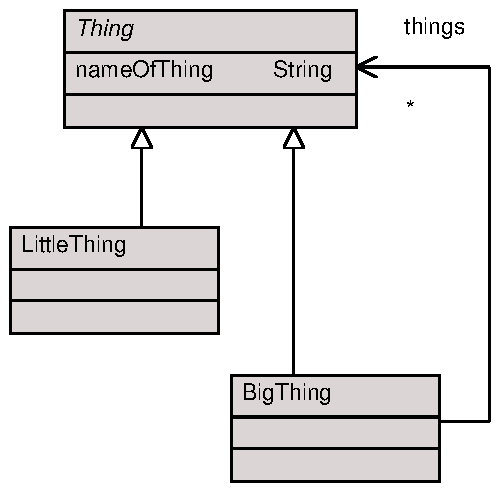
\includegraphics[width=6cm]{Metamodelling/figures/MMExample}
\caption{Visualising concepts and relationships}
\label{classDiagramView}
\end{center}
\end{figure}

The main benefit of a visual syntax is its ability to express
large amounts of detail in an intuitive and understandable form.
Its obvious weakness is that only certain levels of detail can be
expressed beyond which it becomes overly complex and
incomprehensible.

In practice, utilising a mixture of diagrammatical and textual
syntaxes gains the benefits of both forms of representation. Thus,
a language will often use visual notations to present a higher
level view of the model, whilst textual syntax will be used to
capture detailed properties.

\subsection{Abstract Syntax}

The {\em abstract syntax} of a language describes the vocabulary
of concepts provided by the language and how they may be combined
to create models. It consists of a definition of the concepts, the
relationships that exist between concepts and well-formedness
rules that state how the concepts may be legally combined.

Consider a simple state machine language. An abstract syntax model
of this language may include concepts such as State, Transition
and Event. In addition, there will be relationships between
concepts, such as a Transition being related to a source and
target State. Finally, well-formedness rules will be defined that
ensure, for example, that no two transitions may be triggered by
the same event.

It is important to emphasise that a language's abstract syntax is
independent of its concrete syntax and semantics. Abstract syntax
deals solely with the form and structure of concepts in a language
without any consideration given to their presentation or meaning.

\subsection{Semantics}

An abstract syntax conveys little information about what the
concepts in a language actually mean. Therefore, additional
information is needed in order to capture the semantics of a
language. Defining a semantics for a language is important in
order to be clear about what the language represents and means.
Otherwise, assumptions may be made about the language that lead to
its incorrect use. For instance, although we may have an intuitive
understanding of what is meant by a state machine, it is likely
that the detailed semantics of the language will be open to
misinterpretation if they are not defined precisely. What exactly
is a state? What does it mean for transition to occur? What
happens if two transitions leave the same state. Which will be
chosen? All these questions should be captured by the semantics of
the language.

It is critical that semantics should be captured in a way that is
precise and useful to the user of the language. An abstract
mathematical description has little benefit if it cannot be
understood or used. Instead, a semantic definition that provides
rich ways of interacting with the language should be the goal of
the language designer: An executable language should have an
operational semantics that allows it be run; A language which
contains type concepts, such as classes, should permit the
creation of objects according to the rules of instantiation, and
so on.

\subsection{Mappings} In the real world, languages
do not exist in isolation. They will have a relationships to other
languages. This may be via translation (concepts in one language
are translated into concepts in another language); semantic
equivalence (a language may have concepts whose meaning overlaps
with concepts in another language) or abstraction (a language may
be related to another language that is at a different level of
abstraction). Capturing these relationships is an important part
of a language's definition as it serves to place the language in
the context of the world around it. Furthermore, mappings exist
between the internal components of languages, such as between a
concrete and abstract syntax, and are an important part of a
language's architecture (see section \ref{families}).

\subsection{Extensibility} Languages are not static entities: they
change and evolve over time. For instance, new concepts may be
added that enable common patterns of model or code to be expressed
more succinctly, whilst unused elements of the language will
eventually die out. The ability to extend a language in a precise
and well-managed way is vital in order to be able to support
adaptability. It allows the language to adapt to new application
domains and to evolve to meet new requirements. Furthermore,
extensibility enables the commonality and differences between
languages to be precisely captured.

\section{Modelling Languages vs. Programming Languages}
\label{progvsmodel} A strong distinction has traditionally been
made between modelling languages and programming languages (a fact
reflected by the two distinct modelling and programming
communities!). One reason for this is that modelling languages
have been traditionally viewed as having an informal and abstract
semantics whereas programming languages are significantly more
concrete due to their need to be executable.

This is not the case in this book. Here, we view modelling
languages and programming languages as being one and the same.
Both have a concrete syntax, abstract syntax and semantics. If
there is a difference, it is the level of abstraction that the
languages are targeted at. For instance, UML tends to focus on
specification whilst Java emphasises implementation. However, even
this distinction is blurred: Java has been widely extended with
declarative features, such as assertions, whilst significant
inroads have been made towards developing executable versions of
UML.

Another common distinction made between modelling and programming
languages is their concrete syntax. Modelling languages tend to
provide diagrammatical syntaxes, whilst programming languages are
textual. However, the representational choice of a language should
not enforce this distinction. There is nothing to say that a
modelling language cannot have a textual syntax or that
programming language cannot have a visual syntax: it is purely a
matter of representational choice. Indeed there is already a human
readable textual form of UML and tools that provide visual front
ends to programming languages like Java are commonplace.

If modelling languages and programming languages are essentially
the same, why can't the mature techniques used to define
programming languages be used to design modelling languages? The
answer is that they can - indeed many of the techniques presented
here have their foundation in programming language design.
However, there is one important element that is missing from many
approaches to defining programming languages, and that is
unification. It is the ability to define multiple languages that
co-exist in a unified meta-architecture that make metamodelling
such a powerful technology.

Thus, the techniques that are developed in this book are equally
as applicable to programming languages as they are to modelling
languages. A critical failing of modelling languages is that they
have not, until now, been given the precise, executable
definitions that programming languages enjoy.

\section{What is a Metamodel?}

In its broadest sense, a metamodel is a model of a modelling
language. The term "meta" means transcending or above, emphasising
the fact that a metamodel describes a modelling language at a
higher level of abstraction than the modelling language itself.

In order to understand what a metamodel is, it is useful to
understand the difference between a metamodel and a model. Whilst
a metamodel is also a model (as defined in chapter
\ref{lddchapter}), a metamodel has two main distinguishing
characteristics. Firstly, it must capture the essential features
and properties of the language that is being modelled. Thus, a
metamodel should be capable of describing a language's concrete
syntax, abstract syntax and semantics. Note, how we do this is the
major topic of the rest of this book!

Secondly, a metamodel must be part of a {\em metamodel
architecture}. Just as we can use metamodels to describe the valid
models or programs permitted by a language, a metamodel
architecture enables a metamodel to be viewed as a model, which
itself is described by another metamodel. This allows all
metamodels to be described by a single metamodel. This single
metamodel, sometimes known as a meta-metamodel, is the key to
metamodelling as it enables all modelling languages to be
described in a unified way. How metamodels can be {\em described}
by a meta-metamodel is discussed in more detail in section
\ref{metaarch}.

It is important to be aware that there is a good deal of confusion
about what is meant by a metamodel in the literature. Many
standards such as UML \cite{umlspec}, CWM \cite{cwmspec} and MOF
\cite{mofspec} provide `metamodels' that claim to define the
standard, yet they only focus on the abstract syntax of the
languages. They should really be viewed partial metamodels (or
even just models) as they do not provide a complete language
definition.

\section{Why Metamodel?}

As discussed in chapter \ref{lddchapter}, system development is
fundamentally based on the use of languages to capture and relate
different aspects of the problem domain.

The benefit of metamodelling is its ability to describe these
languages in a unified way. This means that the languages can be
uniformly managed and manipulated thus tackling the problem of
language diversity. For instance, mappings can be constructed
between any number of languages provided that they are described
in the same metamodelling language.

Another benefit is the ability to define semantically rich
languages that abstract from implementation specific technologies
and focus on the problem domain at hand. Using metamodels, many
different abstractions can be defined and combined to create new
languages that are specifically tailored for a particular
application domain. Productivity is greatly improved as a result.

\subsection{Metamodels and Tools}

The ability to describe all aspects of a language in a metamodel
is particularly important to tool developers.

Imagine the benefits of loading a metamodel of a language into a
tool that defined all aspects of the language. The tool would
immediately understand everything relating to the presentation and
storage of models or programs in the language, the users'
interaction with and creation of models or programs, and how to
perform semantically rich activities, such as execution, analysis
and testing. Furthermore, any number of other languages could also
be loaded in the same way, enabling the construction of
semantically rich development environments. Because all the
languages are defined in the same way, interoperability between
the tools would be straightforward. This flexibility would not
just be restricted to user level languages. Another example might
be loading an extension to the meta-metamodel, such as a new kind
of mapping language. This language would then be immediately
available to capture mappings between different languages.

Allowing all aspects of tools to be modelled in a single, platform
independent metamodelling language will have big implications for
the software engineering industry. Firstly, the interoperability
and flexibility of tools will be drastically increased. This will
lead to a marketplace for tool metamodels. Metamodels that provide
partial definitions of languages could be easily extended to
provide many other capabilities by vendors with expertise in a
specific modelling domain.

Secondly, rich metamodels will have a significant benefit to the
standards community. As we have argued, there is currently no
means of capturing complete language definitions in existing
metamodelling languages. As a result, standards that use
metamodels to describe the languages they define suffer because
their informal definitions can be interpreted in many ways.
Complete metamodels of standards such as UML would greatly enhance
the rigour by which the standard is implemented and understood -
something that all stakeholders will benefit from.

\section{Where do you find Metamodels?}

Metamodels have been around for many years in a wide variety of
different application domains and under various pseudonyms: "data
model", "language schema", "data schema" are all terms we have
seen. Wherever there is a need to define a language, it is common
to find a metamodel. This is particularly the case for standards,
which by virtue of being a standard must have a precise
definition. Examples include AP233 and SysML (systems
engineering), SPEM (process modelling), OSS (telecoms) and CWM
(data warehousing). The Object Management Group (OMG) has been
particularly involved in their use in the standards arena. One of
the largest metamodels (about 200 pages long) is contained in the
UML specification \cite{umlspec}. With the advent of MDA
\cite{mda} and the increasing need for standardisation across the
systems development community, the number of applications of
metamodels is set to grow significantly.

Finally, although many developers may view metamodels as being
un-connected with their daily work, it is interesting to note that
many are already using metamodels without knowing it! Many
developers have already experienced the benefits of designing
frameworks containing a vocabulary of language concepts. For
example, developers of financial systems will use concepts such as
financial transactions, accounts, and so on. In reality, they are
defining a language for their domain.

\section{Metamodelling Languages}

A metamodel is written in a metamodelling language, which is
described by a meta-metamodel. As described above, the aim is that
the same metamodelling language (and meta-metamodel) is used to
describe any number of different languages. Thus, provided that
the modelling languages have been defined in the same
metamodelling language, it is possible to treat their definitions
in a unified manner. For example, they can be stored and
manipulated in the same way, or related by mappings.

What distinguishes a metamodelling language from a general purpose
programming language like Java or a modelling language like UML?
The answer is that a metamodelling language is a language
specifically designed to support the design of languages. An
essential requirements of a metamodelling language therefore is
its ability to concisely capture all aspects of a modelling
language, including its syntax and semantics.

\noindent The next chapter will examine in detail the required
components of a metamodelling language.

\section{Metamodel Architectures}
\label{metaarch}

A metamodelling language places requirements on there being a
specific metamodelling archictecture. This architecture provides a
framework within which some key features of a metamodel can be
realised. An important property of a metamodel architecture is
that it describes a classification hierarchy. Models written in
the language are {\em instances} of the concepts that are defined
in the metamodel - the structure of the instances is classified by
the metamodel. Furthermore, many  languages have their own notion
of classification (although they need not), and the pattern is
repeated until a point is reached at which further classification
does not occur. This repeating pattern of
classification/instantiation contributes to what is commonly known
as a meta-level architecture - a concept that will be described in
more detail in the next sections.

\subsection{Traditional Metamodel Architecture}

The traditional metamodel architecture, proposed by the original
OMG MOF 1.X standards is based on 4 distinct meta-levels. These
are as follows:

\begin{description}
\item[M0] contains the data of the application (for example, the
instances populating an object-oriented system at run time, or
rows in relational database tables). \item[M1] contains the
application: the classes of an object-oriented system, or the
table definitions of a relational database. This is the level at
which application modeling takes place (the type or model level).
\item[M2] contains the metamodel that captures the language: for
example, UML elements such as Class, Attribute, and Operation.
This is the level at which tools operate (the metamodel or
architectural level). \item[M3] The meta-metamodel that describes
the properties of all metamodels can exhibit. This is the level at
which modeling languages and operate, providing for interchange
between tools.
\end{description}

Each level in this hierarchy represents an instance of a
classifier relationship. As shown in figure \ref{4layer}, elements
at M0 are instances of classes at M1, which themselves can be
viewed as instances of metamodel classes, which can be viewed as
instances of meta-metamodel classes.

\begin{figure}[htb]
\begin{center}
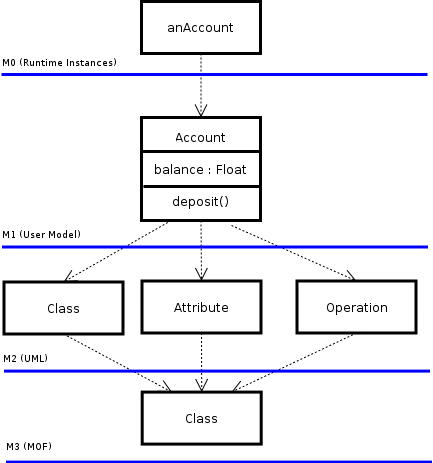
\includegraphics[width=10cm]{Metamodelling/figures/4layer.png}
\caption{Example of the 4 Layer Meta Architecture} \label{4layer}
\end{center}
\end{figure}


The unifying factor in this architecture is the meta-metamodel. It
defines the simplest set of concepts required to define any
metamodel of a language.

\subsection{Golden Braid Metamodel Architecture}
\label{goldenbraid}

Although the 4-layer metamodel is widely cited, its use of
numbering can be confusing. An alterative architecture is the
golden braid architecture \cite{escher}. This architecture
emphasises the fact that metamodels, models and instances are all
relative concepts based on the fundamental property of
instantiation.

The idea was first developed in LOOPS (the early Lisp Object
Oriented Programming System, and then became a feature of both
ObjVLisp \cite{objVlisp} and also CLOS (the Common Lisp Object
System).

Underpinning the golden braid architecture is the relationship
between a Class and an Object. A Class can be instantiated to
create an Object. An Object is said to be an instance of a Class.
This fact can be determined through a distinct operation, of(),
that returns the Class that the Object was created from.

In addition, a Class is also a subclass of Object. This means that
a Class can also be instantiated by another Class: its meta Class.
This relationship is key to the meta-architecture, as it enables
an arbitrary number of meta-levels to be described through the
instantiation relationship.

In practice, there will be a distinct Class that all elements in
the meta-architecture are instances of. This is the
meta-metaclass, which is effectively used to bootstrap the entire
metamodel architecture. This class will be defined as part of the
meta-metamodel (the model of the metamodelling language used to
model all languages).

In terms of the 4-layer metamodel, it is clear that it can be
viewed as the result of stamping out the golden braid architecture
over a number of different levels. Thus, there is no notion of a
meta-metamodel: it is just a metamodel that describes models,
which themselves may be metamodels.

The golden braid architecture offers a great deal of flexibility.
Thus it forms the foundation of the XMF metamodelling language,
which will be presented in chapter \ref{xmfchapter}.

\subsubsection{Meta Object Protocol}

A related aspect of the golden braid architecture is its use of a
meta-object protocol (MOP). A meta-object protocol is a set of
classes and methods that allow a program to inspect the state of,
and alter the behaviour of its meta-metamodel at run-time. These
make it possible to easily adapt the metamodelling language to
support different types of behaviours. For instance, changing the
way that inheritance works, or modifying how the compiler works
without having to change the code for the compiler. This adds
further flexibility to the metamodelling process.

\section{The Metamodelling Process}

The task of creating a metamodel for a language is not a trivial
one. It will closely match the complexity of the language being
defined, so for example, a language containing rich executable
capabilities will be much more complex to define than a simple
static language.

However, there {\em is} a clearly defined process to constructing
metamodels, which does at least make the task a well-defined, if
iterative, process. The process has the following basic steps:

\begin{itemize}
\item defining abstract syntax \item defining well-formedness
rules and meta-operations \item defining concrete syntax \item
defining semantics \item constructing mappings to other languages
\end{itemize}

Much of the remainder of the book will focus on the detail
involved in this process. Initially, we will present the tools
necessary to create metamodels in the first place; the armoury of
metamodelling facilities that is the metamodelling language.

\section{Five levels of Metamodelling}

We are often asked by clients how they can assess the quality of a
metamodel. To help them, we have found the following five levels
to be useful:

\begin{description}
\item [Level 1] This is the lowest level. A simple abstract syntax
model must be defined, which has not been checked in a tool. The
semantics of the language it defines will be informal and
incomplete and there will be few, if any, well-formed rules.
\item [Level 2] At this level, the abstract syntax model will
be relatively complete. A significant number of well-formedness
rules will have been defined, and some or all of the model will
have been checked in a tool. Snapshots of the abstract syntax
model will have been constructed and used to validate its
correctness. The semantics will still be informally defined.
However, there may be more in the way of analysis of the language
semantics.
\item [Level 3] The abstract syntax model will be completely tried
and tested. Concrete syntax will have been defined for the
language, but will only have been partially formalised. Typically,
the concrete syntax will be described in terms of informal
examples of the concrete syntax, as opposed to a precise concrete
syntax model. Some consideration will have been given to the
extensibility of the language architecture, but it will not be
formalised or tested.
\item [Level 4] At level 4, the concrete syntax of the language
will have been formalised and tested. Users will be able to create
models either visually and textually and check that they result in
a valid instance of the abstract syntax model. The language
architecture will have been refactored to facilitate reuse and
extensibility. Models of semantics will have begun to appear.
\item [Level 5] This is the topmost level. All aspects of the
language will have been modelled, including its semantics. The
semantic model will be executable, enabling users of the language
to perform semantically rich operations on models written in the
language, such as simulation, evaluation and execution. The
language architecture will support good levels of reuse, it will
have been proven to do so through real examples. Critically, the
completed metamodel will not be reliant on any external technology
- it will be a fully platform independent and self contained
definition of the language that can be used `as is' to generate or
instantiate tools.
\end{description}

Most of the metamodels we have seen do not achieve a level greater
than 2. Even international standards such as UML do not exceed
level 3. Yet, reaching level 5 must be an aspiration for all
language developers.

\section{Conclusion}

This chapter has outlined some of the key features of system
development languages. All languages have a concrete syntax, which
defines how they are presented, an abstract syntax that describes
the concepts of the language, and a semantics that describes what
the concepts mean. A metamodel is a model of all these different
aspects of a language. Crucially, a metamodel can also be thought
of as a model, written in a metamodelling language, which is
itself is also described by a metamodel. This enables all
metamodels to be described in the same way. This facilitates a
truly unified approach to language definition.
